\section{Entity Relationship Diagram}
\subsection{Entities}
We will have seven entities: user, post, Q\&A post, question, answer, comment, and topic.

A user is any individual writing a post on Ask Us. The user entity will have five attributes: ID, name, email, password, and points. A user's points are the sum of all the points of all their posts. ID will be the primary key.

A post is anything a user writes. This can either be a question, answer, or comment. The post entity wil have four attributes: ID, body, date-time, and points. Here, points is the number of points that have been awarded to any specific post. ID is the primary key.

A Q\&A post is either a question or an answer that a user posts. The Q\&A post entity has no attributes of its own, since it is a weak entity. Its primary key is the post's ID.

A question is what a user would post if he wanted to receive a solution to his inquiry. The question entity has one attribute called title, as well as the attributes it `inherits' from post. Since it is a weak entity, its primary key is the post's ID.

An answer is what a user would post if he wanted to give a solution to a question. The answer entity has a boolean attribute called accepted. Other than that, all the rest of the attributes are `inherited' from post.

A comment is a type of post, and is typically a short piece of text that a user writes beneath any other post. A comment itself has no attributes. Since it is a weak entity, its primary key is the post's ID.

A topic is a way for users to categorize their questions, thus getting better targeted responses. A user can also follow a topic of interest. The topic entity will have three attributes: ID, name, and description. ID will once again be the primary key.

\subsection{Relations}
A user can `follow' a topic. In this relation, there can be many topics a user can follow but it is not mandatory for a user to follow any topic. In the same light, there can be topics followed by any number of users.

A user is related to the posts that they write. In this relation, the user can write anywhere from many to no posts. However, a post must be written by exactly one user.

The comment entity has two relations with the post entity. One relation is called belongs to. This relation represents the fact that a specific comment has a parent post (which may also be a comment). A post can optionally have many comments, but a comment must be a child of exactly one post.

The other relation is an inheritance relation. It is an identifying relation, and is labelled `is a' in figure \ref{erd}. In this relation, a particular comment is related to exactly one post, meaning that this comment entity `extends' that post, because they are in fact the same post. In this relation, a post does not necessarily have to be related to a comment, since not all posts are comments, but if it is, it must be related to exactly one comment.

Since a Q\&A post is also a type of post, it also has an inheritance relation between itself and post. This relation is identical to the inheritance relation between comment and post. Similarly, both question and answer have an identical relation between themselves and Q\&A post.

Answers must also be related to the questions which they answer. A question can have zero to infinitely many answers, yet an answer must be related to exactly one question.

Lastly, questions are related to topics. A question must have at least one topic, and a topic can have zero or more questions related to it.

\subsection{Diagram}

Figure \ref{erd} shows the entity relationship diagram for the database we are to make for Ask Us.

\begin{figure}[htb]
	\centering
	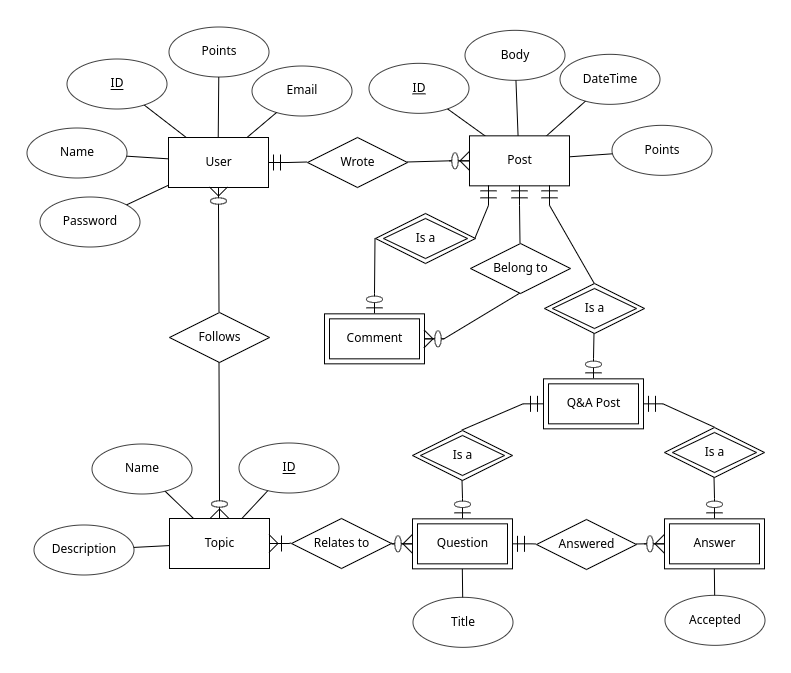
\includegraphics[width=\linewidth]{../../ERD/erd.png}
	\caption{An ERD for the database for Ask Us}
	\label{erd}
\end{figure}
